\documentclass[10pt,fleqn,a4paper]{jsarticle}
\usepackage[dvipdfmx]{graphicx,color}
\usepackage{ascmac,amsmath,amssymb,amstext}
\usepackage{tikz,multicol,float,tikz-3dplot}
\usetikzlibrary{positioning,intersections,calc,arrows.meta,math,angles}
\usepackage{zogeny,ceo,comment}
\newcommand{\ans}[1]{\mbox{\boldmath{$#1$}}}
\renewcommand{\baselinestretch}{1.3} 
\tdplotsetmaincoords{60}{110}%{xy平面からどれだけ上にいるか(90度から-90度)}{z軸中心にどれだけ左右に回転するか}
\title{立教大-社会科学部-過去問演習}
\author{大島}
\begin{document}
\maketitle
\newpage
{\LARGE 過去問演習の意味とは}\\
 受験生が受験勉強をする中で誰しも通るものが,\ans{過去問演習}である.\\
ただし,その過去問演習は,\ans{回数をこなすだけ}の勉強になってはいないだろうか.そこで,私のおすすめの過去問への取り組み方を少し
述べようと思う.\\\\
過去問演習とは,次の目的を達成するために用いるべし.\\

    {\large \noindent\ans{1}.受験校の難易度・傾向を掴む.}\\
    {\large \ans{2}.受験校の教授は,どのような\ans{数学的な発想・考え方をすることを要求しているのか?}を把握する.
    (傾向に合わせた思考をできるようになる.)}\\
    {\large \ans{3}.時間配分を考える.}\\
    {\large \ans{4}.どの程度できれば御の字なのかを把握し,その正答率を目指して解く.}\\
    {\large \ans{5}.自分で採点せず,他の人に添削をお願いする.(自分では,良いように思えても実際,ダメなことがよくある.)}\\
    {\large\ans{6}.過去問演習は,2週目まで.(周回して,受かる気になっているだけ.過去問で出題された問題はほぼ出ない.)}\\
    {\large \ans{7}.良い点が取れなくても落ち込まない.(相性がある.その結果に一喜一憂している暇はない.その時間を勉強に充てよ.)}\\
    {\large \ans{8}.最後まで,自分を信じて取り組むこと.(今,合格圏内にいる者はほとんどいない.(僕も,そうだった)最後まで,諦めない!!)}\\\\

    上にあ挙げたようなことを意識して過去問題演習に取り組むのが良いだろう.\\
    最終局面が迫っています.頑張りましょう.\\
    大島 遙斗
    \newpage
    \tableofcontents
    \newpage
    \section{傾向と対策}
    \begin{center}
        {\LARGE\ans{出題傾向}}
    \end{center}
    \begin{center}
        \begin{tabular}{|c|c|c|}
            \hline
           {}&  \tokeni & \tokesan \\
            \hline
            2023.2/6 & \suB 複利計算 & \suII 微積\\
            \hline
            2023.2/9 & \suA 確率 & \suI\suII 絶対値のついた二次関数,微積\\
            \hline
            2024.2/6 & \suII 微積 & \suC ベクトル\\
            \hline 
            2024.2/9 & \suB 漸化式 & \suI\suII 二次関数と微積\\
            \hline
            2025.2/6 & \suA\suB 確率漸化式 & \suII 微積\\
            \hline
            2025.2/9 & \suII 三角関数と図形の融合問題 & \suII 微積\\
            \hline
        \end{tabular}
    \end{center}
    \begin{itembox}   
[c]{\kagil\kagil\enpitu \ans{入試の要}\kagir\kagir}
・立教大学の文系数学の問題は難易度は,一貫して\ans{入試基礎〜入試標準}で推移している.難問は滅多に出題されず入試標準レベルの数学を
どれだけ習得できているかが合否を分けていると考えられる.\\
なので,日頃の演習は典型問題を手際よく解けるようになるのはもちろんのこと,標準レベルの問題を解くのにも慣れておく必要がある.\\
・上の表から分かるように,\ans{微積}は必ず出題される.微積の攻略は必須である.また,微積分野の問題は難易度はさほど高くないので確実
に得点したい.\\
・一方,小問集合で稀に解きにく問題が混ざっていることがある.なので,大問全体を見渡してから解答方針を決定するのが良いだろう.\\
・これらの理由から,選抜は\ans{高得点勝負}になると推測される.英語は独自の試験がにないため,皆安定しているだろう.そう考えると,
\ans{社会科}と\ans{数学}でどれだけミスを抑えることができるかが勝敗の分かれ目となるだろう.
    \end{itembox}
    \newpage
    \section{2023年度(2月6日実施)}
     \begin{center}
        2023年度
    \end{center}
\begin{center}
        

    {\LARGE \ans{A 数 学 問 題}}
    \end{center}
    \begin{center}
        \ans{注 意}
        \end{center}
            
        
        
            \noindent1.試験開始の指示があるまでこの問題冊子を開いてはいけません。\\
            2.解答用紙はすべて\ans{黒鉛筆または黒のシャープペンシル}で記入することになっています。黒鉛筆・消しゴムを忘れた人は
            監督に申し出てください。(万年筆・ボールペン・サインペンなどを使用してはいけません。)\\
            3.この問題用紙は\ans{10ページ}までとなっています。試験開始後,ただちにページ数を確認してください。なお,問題番号は
            \tokeichi 〜\tokesan となっています。\\
            4.解答用紙にはすでに受験番号が記入されていますので,出席表の氏名欄に\ans{氏名}のみを記入してください。
            なお,出席表は切り離さないでください。\\
            5.解答は,解答用紙の指定された場所に記入して,その他の部分には何も書いてはいけません。\\
            6.解答用紙を折り曲げたり,破ったり,傷つけたりしないように注意してください。\\
            7.計算には,この問題の余白部分を使ってください。\\
            8.この問題冊子は持ち帰ってください。
            \newpage
\noindent{\LARGE\tokeichi.} 下記の空欄ア〜キにあてはまる数または式を解答用紙の所定欄に記入せよ.\\\\
$\tokeiichi  関数y=4\cos^2\theta-4\sin\theta-5の最小値は\Bc{ア}である.\\\\
\tokeini  2つの実数x,yがx^2+y^2=1を満たすとき,z=2x+yのとりうる値の範囲は\Bc{イ}である.\\\\
\tokeisan  三角形\mathrm{ABC}において\mathrm{AB}=\mathrm{AC}=4,\mathrm{BC}=6とする.\mathrm{AB}上の点\mathrm{P}
が\mathrm{CP}=5を満たすとき,\mathrm{AP}=\Bc{ウ}である.\\\\
\tokeishi  大小2個のさいころを同時に投げる.大きいさいころの出た目をa,小さいサイコロの出た目をbとするとき,\dfrac{a}{b}が整数
になる確率は\Bc{ウ}である.\\\\
\tokeigo  tを実数とする.座標空間において,3点\mathrm{O}\p{0,0,0},\mathrm{A}\p{1,0,2},\mathrm{B}\p{2,-1,0}の定める
平面\mathrm{OAB}上に点\mathrm{C}\p{1+t,t,1-t}があるとき,t=\Bc{オ}である.\\\\
\tokeiroku  2次式f(x)がf(f(x))=f(x)^2+1を満たすとき,f(x)=\Bc{カ}である.\\\\
\tokeishichi  座標平面の3つの部分空間$
\begin{align*}
        &A=\B{(x,-2x+2)|xは実数,x<0}\\
        &B=\B{(x,2x+2)|xは実数,x\geq0}\\
        &C=\B{(x,-x+3)|xは実数}
    \end{align*}
に対し,$\p{A\cup B}\cap Cに属する点の座標をすべて求めると\Bc{キ}である.$
    \newpage
    \begin{center}
        計算用紙
    \end{center}
    \newpage
    \noindent{\LARGE\tokeni.} $1年目の初めに新規に100万円を預金し,2年目以降の毎年初めに12万円を追加で預金する.ただし,毎年の
    終わりに,その時点での預金額の8%が利子として預金に加算される.自然数nに対して,n年目の終わりに利子が加算された後の預金額をS_n万円
    とする.このとき,次の問\tokeiichi 〜\tokeigo に答えよ.ただし,\log_{10}2=0.3010,\log_{10}3=0.4771 とする.解答欄には,
    \tokeiichi,\tokeini については答えのみを,\tokeisan 〜\tokeigo については答えだけでなく途中経過も書くこと.\\\\
    \tokeiichi  S_1,S_2をそれぞれ求めよ.\\\\
    \tokeini  S_{n+1}をS_nを用いて表せ.\\\\
    \tokeisan  S_nをnを用いて表せ.\\\\
    \tokeishi  \log_{10}10.8を求めよ.\\\\
    \tokeigo  S_n>513を満たす最小の自然数nを求めよ.$
\newpage
\begin{center}
    計算用紙
\end{center}
\newpage
\noindent{\LARGE\tokesan.} $pを正の実数とする.\mathrm{O}を原点とする座標平面上の放物線C:y=\dfrac{1}{4}x^2上の点
\mathrm{P}\p{p,\dfrac{1}{4}p^2}における接線をl,\mathrm{P}を通りx軸に垂直な直線をmとする.また,m上の点\mathrm{Q}\p{p,-1}
を通り,lに垂直な直線をnとし,lとnの交点を\mathrm{R}とする.さらに,lに関して\mathrm{Q}と対称な点を\mathrm{S}とする.このとき,
次の問\tokeiichi 〜\tokeigo に答えよ.解答欄には,\tokeiichi については答えのみを,\tokeini 〜\tokeigo については
答えだけでなく途中経過も書くこと.\\\\
\tokeiichi  lの方程式をpを用いて表せ.\\\\
\tokeini  nの方程式および\mathrm{R}の座標をそれぞれpを用いて表せ.\\\\
\tokeisan  \mathrm{S}の座標を求めよ.\\\\
\tokeishi  lを対称軸として,lに関してmと対称な直線m'の方程式をpを用いて表せ.また,m'とCの交点のうち\mathrm{P}と異なる点を\mathrm{T}
とするとき,\mathrm{T}のx座標をpを用いて表せ.\\\\
\tokeigo  \tokeishi の\mathrm{T}に対して,線分\mathrm{ST},\mathrm{OS}およびCで囲まれた部分の面積をpを用いて表せ.$
\newpage
\begin{center}
    計算用紙
\end{center}
\newpage
\begin{center}
    \underline{色々メモするスペース}
\end{center}
\newpage
\section{2023年度(2月9日実施)}
  \begin{center}
        2023年度
    \end{center}
    \begin{center}
        

    {\LARGE \ans{C 数 学 問 題}}
    \end{center}
    \begin{center}
        \ans{注 意}
        \end{center}
            
        
        
            \noindent1.試験開始の指示があるまでこの問題冊子を開いてはいけません。\\
            2.解答用紙はすべて\ans{黒鉛筆または黒のシャープペンシル}で記入することになっています。黒鉛筆・消しゴムを忘れた人は
            監督に申し出てください。(万年筆・ボールペン・サインペンなどを使用してはいけません。)\\
            3.この問題用紙は\ans{18ページ}までとなっています。試験開始後,ただちにページ数を確認してください。なお,問題番号は
            \tokeichi 〜\tokesan となっています。\\
            4.解答用紙にはすでに受験番号が記入されていますので,出席表の氏名欄に\ans{氏名}のみを記入してください。
            なお,出席表は切り離さないでください。\\
            5.解答は,解答用紙の指定された場所に記入して,その他の部分には何も書いてはいけません。\\
            6.解答用紙を折り曲げたり,破ったり,傷つけたりしないように注意してください。\\
            7.計算には,この問題の余白部分を使ってください。\\
            8.この問題冊子は持ち帰ってください。
\newpage
\noindent{\LARGE\tokeichi.} 下記の空欄ア〜クにあてはまる数または式を解答用紙の所定欄に記入せよ.\\\\
$\tokeiichi  円に内接する\mathrm{AB}=3,\mathrm{BC}=6,\mathrm{CD}=5,\mathrm{DA}=2である四角形\mathrm{ABCD}において,
\cos A=\Bc{ア}である.\\\\
\tokeini  整式\p{x+1}^{2023}をx^2で割った余りは\Bc{イ}である.\\\\
\tokeisan  \log_62=aに対して,3^{\frac{1}{1-a}}は整数であり,その値は\Bc{ウ}である.\\\\
\tokeishi  座標平面上の3点\mathrm{O}(0,0) ,\mathrm{A}(4,2),\mathrm{B}(-6,6)を頂点とする三角形\mathrm{OAB}の外心の座標
は\Bc{エ}である.\\\\
\tokeigo  z=\dfrac{\sqrt{3}+i}{2}に対して,z^6=a+biとする.このとき,a=\Bc{オ},b=\Bc{カ}である.ただし,iは虚数単位とし,a,b
は実数とする.\\\\
\tokeiroku  \left|\vec{a}\right|=3,\left|\vec{b}\right|=4,\left|\vec{a}+\vec{b}\right|=\sqrt{17}を満たす2つのベクトル
\vec{a},\vec{b}が作る平行四辺形の面積は\Bc{キ}である.\\\\
\tokeishichi  数列\B{a_n}が$
\begin{center}
    $a_1=0,a_{n+1}=-a_n+3 (n=1,2,3,\cdots)$
\end{center}
を満たすとする.$自然数nを2で割った商をmとしたとき,\wa{k=1}{n}a_k をmを用いて表すと\Bc{ク}である.$
\newpage
\begin{center}
    計算用紙
\end{center}
\newpage
\noindent{\LARGE\tokeni.} A,B,C,Dの$4人でじゃんけんをするゲームを行う.1回のじゃんけんで1人でも勝者が出た場合は,ゲームを
終了する.だれも勝たずあいこになる場合は,4人でもう一度じゃんけんをし,勝者げでるまでじゃんけんを繰り返す.次の問\tokeiichi 〜\tokeigo
に答えよ.解答欄には,\tokeiichi については答えのみを,\tokeini 〜\tokeigo については答えだけでなく途中経過も書くこと.$\\\\
$\tokeiichi  1回目のじゃんけんで,$Aだけが勝つ確率を求めよ.\\\\
\tokeini  $1$回目のじゃんけんで,Aを含む$2人だけが勝つ確率を求めよ.\\\\
\tokeisan  1回目のじゃんけんで,\mathrm{A}が勝者に含まれる確率を求めよ.\\\\
\tokeishi  1回目のじゃんけんで,だれも勝たずあいこになる確率を求めよ.\\\\
\tokeigo  2回目のじゃんけんで,ゲームが終了する確率を求めよ.$
\newpage
\begin{center}
    計算用紙
\end{center}
\newpage
\noindent{\LARGE\tokesan.} $0<t<2とし,座標平面上の曲線C:y=\left|x^2+2x\right|上の点\mathrm{A}(-2,0)を通る傾きtの直線
をlとする.Cとlの,\mathrm{A}以外の異なる2つの共有点を\mathrm{P},\mathrm{Q}とする.ただし,\mathrm{P}のx座標は,\mathrm{Q}
のx座標より小さいとする.このとき,次の問\tokeiichi 〜\tokeigo に答えよ.解答欄には,\tokeiichi については答えのみを,\tokeini 〜
\tokeigo については答えだけでなく途中経過も書くこと.\\\\
\tokeiichi  \mathrm{P},\mathrm{Q}のx座標をそれぞれtを用いて表せ.\\\\
\tokeini  線分\mathrm{AP}とCで囲まれた部分の面積S_1(t)をtを用いて表せ.\\\\
\tokeisan  線分\mathrm{PQ}とCで囲まれた部分の面積S_2(t)をtを用いて表せ.\\\\
\tokeishi  線分\mathrm{AQ}とCで囲まれた2つの部分の面積の和S(t)をtを用いて表せ.また,S(t)の導関数S'(t)を求めよ.\\\\
\tokeigo  tが0<t<2を動くとき,\tokeishi のS(t)を最小にするようなtの値を求めよ.$
\newpage
\begin{center}
    計算用紙
\end{center}
\newpage
\begin{center}
\underline{色々メモするスペース}
\end{center}
\newpage
    \section{2024年度(2月6日実施)}
    \begin{center}
        2024年度
    \end{center}
    \begin{center}
        

    {\LARGE \ans{A 数 学 問 題}}
    \end{center}
    \begin{center}
        \ans{注 意}
        \end{center}
            
        
        
            \noindent1.試験開始の指示があるまでこの問題冊子を開いてはいけません。\\
            2.解答用紙はすべて\ans{黒鉛筆または黒のシャープペンシル}で記入することになっています。黒鉛筆・消しゴムを忘れた人は
            監督に申し出てください。(万年筆・ボールペン・サインペンなどを使用してはいけません。)\\
            3.この問題用紙は\ans{26ページ}までとなっています。試験開始後,ただちにページ数を確認してください。なお,問題番号は
            \tokeichi 〜\tokesan となっています。\\
            4.解答用紙にはすでに受験番号が記入されていますので,出席表の氏名欄に\ans{氏名}のみを記入してください。
            なお,出席表は切り離さないでください。\\
            5.解答は,解答用紙の指定された場所に記入して,その他の部分には何も書いてはいけません。\\
            6.解答用紙を折り曲げたり,破ったり,傷つけたりしないように注意してください。\\
            7.計算には,この問題の余白部分を使ってください。\\
            8.この問題冊子は持ち帰ってください。





\newpage


    
制限時間:60分 解答用紙:A3一枚\\\\
{\LARGE \tokeichi.} 下記の空欄ア〜コにあてはまる数または式を解答用紙の所定欄に記入せよ.\\\\
$\tokeiichi  1\leq x\leq8の範囲において,関数y=\p{\log_2x}^2-8\log_2x-20はx=\Bc{ア}のときに最小値\Bc{イ}をとる.\\\\
\tokeini  等式$
\begin{center}
    $\dfrac{3x^2-x+4}{\p{x+1}^3}=\dfrac{a}{\p{x+1}^3}+\dfrac{b}{\p{x+1}^2}+\dfrac{c}{x+1}$
\end{center}
が$xについての恒等式となるような定数a,b,cは,a=\Bc{ウ},b=\Bc{エ},c=\Bc{オ}である.\\\\
\tokeisan  さいころを3回投げて出る目をすべてかけた数が4の倍数となる確率は\Bc{カ}である.\\\\
\tokeishi  \theta=\dfrac{\pi}{12}のとき,\dfrac{1}{\tan\theta}-\tan\theta の値は\Bc{キ}である.\\\\
\tokeigo  初項と第2項がそれぞれa_1=1,a_2=1である数列\B{a_n}は,n\geq2のとき等式$
\begin{center}
    $a_{n+1}=a_1+a_2+\cdots+a_n$
\end{center}
をみたす.$n\geq3のとき,a_nをnを用いて表すとa_n=\Bc{ク}である.\\\\
\tokeiroku  0\leq x\leq1の範囲においてf(x)\geq0である2次関数f(x)=ax^2+bは,等式$
\begin{center}
    $f(x)\p{\dint{0}{1}f(t)dt}=x^2+5$
\end{center}
を満たす.$このとき,定数a,bは,a=\Bc{ケ},b=\Bc{コ}である.$
\newpage
\begin{center}
    計算用紙
\end{center}

\newpage
\noindent{\LARGE\tokeni.} $p,qを正の実数とする.座標平面上に放物線C:y=-x^2がある.C上の点\mathrm{P}(p,-p^2)におけるCの
接線をl,点\mathrm{Q}(-q,-q^2)におけるCの接線をmとする.また,lとmの交点を\mathrm{R}とする.このとき,次の問\tokeiichi〜
\tokeiroku に答えよ.解答欄には,\tokeiichi,\tokeini,\tokeigo については答えのみを,\tokeisan,\tokeishi,\tokeiroku 
については答えだけでなく途中経過も書くこと.\\\\
\tokeiichi  l,mの方程式を求めよ.\\\\
\tokeini  \mathrm{R}の座標をp,qを用いて表せ.\\\\
\tokeisan  \mathrm{Q}とlの距離dをp,qを用いて表せ.\\\\
\tokeishi  三角形\mathrm{PQR}の面積Sをp,qを用いて表せ.\\\\
\tokeigo  lとmが直交するとき,qをpを用いて表せ.\\\\
\tokeiroku  lとmが直交するとき,\tokeishi の面積Sの最小値を求めよ.また,そのときのpの値を求めよ.$

\newpage
\begin{center}
    計算用紙
\end{center}
\newpage
\noindent{\LARGE\tokesan.} $三角形\mathrm{OAB}において,\mathrm{OA}=5,\mathrm{OB}=7,\mathrm{AB}=8とする.また,
\mathrm{O}を中心とする半径rの円Cが直線\mathrm{AB}上の点\mathrm{D}で接している.さらに,\mathrm{A}からCへ引いた接線とCとの
交点を\mathrm{E}とする.ただし,\mathrm{E}は\mathrm{D}と異なる点とする.\Vec{OA}=\vec{a},\Vec{OB}=\vec{b}とおくとき,
次の問\tokeiichi 〜\tokeigo に答えよ.解答欄には,\tokeiichi については答えのみを,\tokeini 〜\tokeigo については,
答えだけでなく途中経過も書くこと.\\\\
\tokeiichi  内積\vec{a}\cdot\vec{b}を求めよ.\\\\
\tokeini  \Vec{OD} を\Vec{OD}=(1-t)\vec{a}+t\vec{b}と表すとき,定数tの値を求めよ.\\\\
\tokeisan  rの値を求めよ.\\\\
\tokeishi  \mathrm{D}から直線\mathrm{OA}へ下ろした垂線を\mathrm{DH}とする.\Vec{OH}を\vec{a}を用いて表せ.\\\\
\tokeigo  \Vec{OE}を\Vec{OE}=p\vec{a}+q\vec{b}と表すとき,定数p,qの値をそれぞれ求めよ.$

\newpage
\begin{center}
    計算用紙
\end{center}
\newpage
\begin{center}
    \underline{色々メモするスペース}
\end{center}
\newpage
\section{2024年度(2月9日実施)}
\begin{center}
        2024年度
    \end{center}
    \begin{center}
        

    {\LARGE \ans{C 数 学 問 題}}
    \end{center}
    \begin{center}
        \ans{注 意}
        \end{center}
        \noindent1.試験開始の指示があるまでこの問題冊子を開いてはいけません。\\
            2.解答用紙はすべて\ans{黒鉛筆または黒のシャープペンシル}で記入することになっています。黒鉛筆・消しゴムを忘れた人は
            監督に申し出てください。(万年筆・ボールペン・サインペンなどを使用してはいけません。)\\
            3.この問題用紙は\ans{34ページ}までとなっています。試験開始後,ただちにページ数を確認してください。なお,問題番号は
            \tokeichi 〜\tokesan となっています。\\
            4.解答用紙にはすでに受験番号が記入されていますので,出席表の氏名欄に\ans{氏名}のみを記入してください。
            なお,出席表は切り離さないでください。\\
            5.解答は,解答用紙の指定された場所に記入して,その他の部分には何も書いてはいけません。\\
            6.解答用紙を折り曲げたり,破ったり,傷つけたりしないように注意してください。\\
            7.計算には,この問題の余白部分を使ってください。\\
            8.この問題冊子は持ち帰ってください。








\newpage
\noindent{\LARGE\tokeichi.} 下記の空欄ア〜クにあてはまる数を解答用紙の所定欄に記入せよ.\\\\
$\tokeiichi  2進数aをa_{(2)}と表す.1011_{(2)}\times11_{(2)}+1111_{(2)}を計算した結果を10進数で表すと\Bc{ア} である.\\\\
\tokeini  袋の中に赤玉と白玉があわせて20個入っている.この袋の中から同時に2つの玉を取り出すとき,取り出した玉が2個とも赤である
確率は\dfrac{21}{38}である.このとき,はじめに袋に入っていた赤玉は\Bc{イ}個である.\\\\
\tokeisan  三角形\mathrm{ABC}において,\mathrm{AB}=3,\mathrm{BC}=4,\mathrm{CA}=2とする.線分\mathrm{BC} の中点
\mathrm{M}とするとき,線分\mathrm{AM} の長さは\Bc{ウ} である.\\\\
\tokeishi  x+\dfrac{1}{x}=-3であるとき,x^3+\dfrac{1}{x^3}=\Bc{ウ} である.\\\\
\tokeigo  -3\leq x\leq3において,関数f(x)=x^3+2x^2-4xの最小値は\Bc{オ} である.\\\\
\tokeiroku  座標空間において,点\mathrm{A}(-10,-3,8)を通り,ベクトル\vec{a}=(1,2,-2)に平行な直線と,xy平面との交点の
座標は(\Bc{カ},\Bc{キ},\Bc{ク})である.
$
\newpage
\begin{center}
    計算用紙
\end{center}
\newpage
\noindent{\LARGE\tokeni.} 次のように定められる正の数からなる数列$\B{a_n}がある.$
\begin{center}
    $a_1=1,a_2=2,a_{n+2}=\sqrt{\dfrac{a^3_{n+1}}{2a_n}} (n=1,2,3,\cdots)$
\end{center}
このとき,次の問$\tokeiichi 〜\tokeigo に答えよ.解答欄には,\tokeiichi,\tokeini については答えのみを,\tokeisan 〜\tokeigo
については答えだけでなく途中経過も書くこと.\\\\
\tokeiichi  a_3=2^x,a_4=2^y,a_5=2^zと表すとき,x,y,zの値をそれぞれ求めよ.\\\\
\tokeini  b_n=\dfrac{a_{n+1}}{a_n}(n=1,2,3,\cdots)とくとき,b_{n+1}をb_nを用いて表せ.\\\\
\tokeisan  \tokeini で定めた数列\B{b_n}に対して,c_n=\log_2b_n(n=1,2,3,\cdots)によって定められる数列\B{c_n}の一般項
を求めよ.\\\\
\tokeishi  \tokeisan で定めた数列\B{c_n}に対して,S_n=\wa{k=1}{n}c_kをnを用いて表せ.\\\\
\tokeigo  数列\B{a_n}の一般項をa_n=2^{d_n}と表す. \tokeishi の結果を用いて,d_nをnを用いて表せ.$
\newpage
\begin{center}
    計算用紙
\end{center}
\newpage
\noindent{\LARGE\tokesan.} $p,qを実数とする.座標平面上に放物線C:y=x^2+2px+qと,2つの直線\ell :y=-x+\dfrac{3}{4},
m:y=2xがある.このとき,以下の問\tokeiichi 〜\tokeigo に答えよ.解答欄には,\tokeini については答えのみを,\tokeiichi と
\tokeisan 〜\tokeigo については答えだけでなく途中経過も書くこと.\\\\
\tokeiichi  Cが\ell に接するとき,qをpを用いて表せ.\\\\
\tokeini  Cが\ell に接するとき,Cの頂点の座標をpを用いて表せ.\\\\
\tokeisan  Cが\ell とx軸の両方に接するとき,Cの方程式を求めよ.また,そのときのCと\ell の頂点のx座標を求めよ.\\\\
\tokeishi  Cが\ell とmの両方に接するとき,Cの方程式を求めよ.また,そのときのCと\ell の接点のx座標を求めよ.\\\\
\tokeigo  \tokeisan で求めたCをC_1,\tokeishi で求めたCをC_2とする.このとき,C_1,C_2,\ell で囲まれた部分の面積Sを
求めよ.$
\newpage
\begin{center}
    計算用紙
\end{center}
\newpage
\begin{center}
    \underline{色々メモするスペース}

\end{center}
\newpage
\section{2025年度(2月6日実施)}


\begin{center}
        2025年度
    \end{center}
    \begin{center}
        

    {\LARGE \ans{A 数 学 問 題}}
    \end{center}
    \begin{center}
        \ans{注 意}
        \end{center}
        \noindent1.試験開始の指示があるまでこの問題冊子を開いてはいけません。\\
            2.解答用紙はすべて\ans{黒鉛筆または黒のシャープペンシル}で記入することになっています。黒鉛筆・消しゴムを忘れた人は
            監督に申し出てください。(万年筆・ボールペン・サインペンなどを使用してはいけません。)\\
            3.この問題用紙は\ans{42ページ}までとなっています。試験開始後,ただちにページ数を確認してください。なお,問題番号は
            \tokeichi 〜\tokesan となっています。\\
            4.解答用紙にはすでに受験番号が記入されていますので,出席表の氏名欄に\ans{氏名}のみを記入してください。
            なお,出席表は切り離さないでください。\\
            5.解答は,解答用紙の指定された場所に記入して,その他の部分には何も書いてはいけません。\\
            6.解答用紙を折り曲げたり,破ったり,傷つけたりしないように注意してください。\\
            7.計算には,この問題の余白部分を使ってください。\\
            8.この問題冊子は持ち帰ってください。
    \newpage

\noindent{\LARGE\tokeichi.} 下記の空欄ア〜クにあてはまる数または式を解答用紙の所定欄に記入せよ.\\\\
$\tokeiichi  x+y=\sqrt{5},xy=1のとき,x^4+y^4=\Bc{ア}である.\\\\
\tokeini  0\leq x<2\pi のとき,\sqrt{2}\sin\p{x+\dfrac{\pi}{4}}+2\cos xの最大値は\Bc{イ}である.\\\\
\tokeisan  等式\log_2x=2\log_x4を満たす実数xを全て求めるとx=\Bc{ウ}である.\\\\
\tokeishi  三角形\mathrm{ABC}において,\mathrm{AB}=1,\mathrm{AC}=\dfrac{\sqrt{2}}{2},
\Vec{AB}\cdot\Vec{AC}=\dfrac{1}{2}とする.辺\mathrm{AB}を1:3に内分する点をDとし,辺\mathrm{AC}を
p:1-pに内分する点を\mathrm{E}とする.ただし,実数pは0<p<1を満たすとする.直線\mathrm{BE}と\mathrm{CD}が
直交するとき,p=\Bc{ウ}である.\\\\
\tokeigo  実数aは定数とし,f(x)=x^2-4x+9,g(x)=axとする.すべての実数xに対して\\f(x)\geq g(x)が成り立つような
aの値の範囲は\Bc{オ}である.\\\\
\tokeiroku  実数a,bは定数とする.3次関数f(x)=x^3+ax^2+bx+2がx=-1とx=\dfrac{1}{3}のそれぞれで極値をとるとき,
a=\Bc{カ},b=\Bc{キ}である.このとき,f(x)の極大値は\Bc{ク}である.$
\newpage
\begin{center}
    計算用紙
\end{center}
\newpage
{\LARGE\tokeni.} $nを1以上の整数とする.箱の中に1から7までの数字が1つずつ書かれた7枚のカードがある.
ただし,異なるカードには異なる数字が書かれたいるとする.$\\
\begin{center}
    \fbox{1}  \fbox{2}  \fbox{3}  \fbox{4}  \fbox{5}  \fbox{6}  \fbox{7}
\end{center}
$「この箱から1枚のカードを無作為に取り出し,そのカードに書かれた数字を記録してからカードを箱の中に戻す」という操作をn回
繰り返す.記録されたn個の数字の和が偶数となる確率をp_nとする.このとき,次の問\tokeiichi 〜\tokeigo に答えよ.
解答欄には,\tokeiichi については答えのみを,\tokeini 〜\tokeigo については答えだけでなく途中経過も書くこと.$\\\\
$\tokeiichi  p_1,p_2を求めよ.\\\\
\tokeini  p_3を求めよ.\\\\
\tokeisan  p_{n+1}をp_nを用いて表せ.\\\\
\tokeishi  p_nをnを用いて表せ.\\\\
\tokeigo  S_n=\wa{k=1}{n}p_kをnを用いて表せ.$
\newpage
\begin{center}
    計算用紙
\end{center}
\newpage
\noindent{\LARGE\tokesan.} $実数a,bは定数とする.2次関数f(x)=x^2+ax+bに対して,座標平面上の放物線CをC:y=f(x)とする.
C上の点\mathrm{P}を\mathrm{P}\p{2\sqrt{2},f(2\sqrt{2})}とし,また,Cとy軸の交点を\mathrm{Q}とする.さらに,円D:
x^2+y^2=1上の点\mathrm{R}\p{\dfrac{\sqrt{2}}{2},-\dfrac{\sqrt{2}}{2}}におけるDの接線を\ell とする.このとき,
次の問\tokeiichi 〜\tokeigo に答えよ.解答欄には,\tokeiichi,\tokeini については答えのみを,\tokeisan 〜\tokeigo に
ついては答えだけでなく途中経過も書くこと.\\\\
\tokeiichi  \ell の方程式を求めよ.\\\\
\tokeini  \ell がCと接するとき,bをaを用いて表せ.\\\\
\tokeisan  \ell が\mathrm{P}においてCと接するとき,a,bの値をそれぞれ求めよ.\\\\
\tokeishi  a,bを\tokeisan で求めた値とする.また,\ell とy軸の交点を\mathrm{S}とする.このとき,$
\begin{center}
    線分SP,  $Cの0\leq x\leq2\sqrt{2}の部分,  線分$QS
\end{center}
で囲まれる図形の面積$X$を求めよ.\\\\
$\tokeigo  a,bを\tokeisan で求めた値とする.また,D上の点\mathrm{T}を\mathrm{T}(0,1)とする.このとき,$
\begin{center}
    線分PR,  $Cの0\leq x\leq2\sqrt{2}の部分$,  線分QT,  Dの弧TR
\end{center}
で囲まれる図形の面積$Y$を求めよ.ただし,弧TRは$x\geq0にあるとする.$
\newpage
\begin{center}
    計算用紙
\end{center}
\newpage
\begin{center}
    \underline{色々メモするスペース}
\end{center}
\newpage
\section{2025年度(2月9日実施)}
\begin{center}
        2025年度
    \end{center}
    \begin{center}
        

    {\LARGE \ans{C 数 学 問 題}}
    \end{center}
    \begin{center}
        \ans{注 意}
        \end{center}
        \noindent1.試験開始の指示があるまでこの問題冊子を開いてはいけません。\\
            2.解答用紙はすべて\ans{黒鉛筆または黒のシャープペンシル}で記入することになっています。黒鉛筆・消しゴムを忘れた人は
            監督に申し出てください。(万年筆・ボールペン・サインペンなどを使用してはいけません。)\\
            3.この問題用紙は\ans{50ページ}までとなっています。試験開始後,ただちにページ数を確認してください。なお,問題番号は
            \tokeichi 〜\tokesan となっています。\\
            4.解答用紙にはすでに受験番号が記入されていますので,出席表の氏名欄に\ans{氏名}のみを記入してください。
            なお,出席表は切り離さないでください。\\
            5.解答は,解答用紙の指定された場所に記入して,その他の部分には何も書いてはいけません。\\
            6.解答用紙を折り曲げたり,破ったり,傷つけたりしないように注意してください。\\
            7.計算には,この問題の余白部分を使ってください。\\
            8.この問題冊子は持ち帰ってください。
\newpage
\noindent{\LARGE\tokeichi.} 下記の空欄ア〜コにあてはまる数または式を解答用紙の所定欄に記入せよ.\\\\
$\tokeiichi  2^{1-3x}\geq\p{\dfrac{1}{\sqrt{2}}}^x を満たす実数xの範囲は\Bc{ア}である.\\\\
\tokeini  赤玉3個と白玉4個を無作為に1列に並べるとき,白玉が両端にある確率は\Bc{イ}である.\\\\
\tokeisan   x,y,zは実数であり,x<yを満たすとする.3つの数3,x,yがこの順に等差数列となり,さらに,4つの数4,x,y,z がこの順に
等差数列となるとき,x=\Bc{ウ},y=\Bc{エ},z=\Bc{オ}である.\\\\
\tokeishi  実数zは定数とする.座標平面上の2つの直線(a+1)x+ay=1,ax+(a+2)y=2 がただ1つの交点をもつためのa条件は\Bc{カ}である.\\\\
\tokeigo  定積分\dint{0}{2}(x+1)|x-1|dx の値は\Bc{キ}である.\\\\
\tokeiroku  空間ベクトル\vec{p}=(x,y,z)は\vec{a}=(1,0,-2)と\vec{b}=(0,3,2)の両方に垂直であり,
\left|\vec{p}\right|かつz>0を満たしている.このとき,\vec{p}=(\Bc{ク},\Bc{ケ},\Bc{コ})である.$
\newpage
\begin{center}
    計算用紙
\end{center}
\newpage
\noindent{\LARGE\tokeni.} $p,qを正の実数とする.原点を\mathrm{O}とする座標平面上に点\mathrm{A}(1,0),
点\mathrm{P}\p{p,\dfrac{1}{p}},点\mathrm{Q}\p{q,\dfrac{2}{q}}がある.\Kaku{AOP}=\alpha,\Kaku{AOQ}=\beta とおき,
\mathrm{P,Q}は\alpha<\beta を満たしながら動くものとする.三角形\mathrm{OPQ}の面積を\mathrm{S}とし,また,T=\tan\p{\beta-\alpha}
とおく.以下の問\tokeiichi 〜\tokeigo に答えよ.解答欄には,\tokeiichi,\tokeini については答えのみを,\tokeisan 〜\tokeigo
については答えだけでなく途中経過も書くこと.\\\\
\tokeiichi  \cos\alpha,\sin\alpha をそれぞれpを用いて表せ.また,\cos\alpha,\sin\beta をそれぞれqを用いて表せ.\\\\
\tokeini  Tをp,qを用いて表せ.\\\\
\tokeisan  Sをp,qを用いて表せ.\\\\
\tokeishi  t=pqとおく.\dfrac{S}{T}を用いて表せ.\\\\
\tokeigo  \dfrac{S}{T}の最小値を求めよ.$
\newpage
\begin{center}
    計算用紙
\end{center}
\newpage
\noindent{\LARGE\tokesan.} $kを実数とする.3次関数f(x)=x^3-x^2+1に対して,座標平面上の曲線CをC:y=f(x)とする.また,C上の点
\mathrm{P}(1,1)を通り,傾きがkである直線を\ell とする.このとき,次の問\tokeiichi 〜\tokeiroku に答えよ.解答欄には,
\tokeiichi 〜\tokeisan については答えのみを,\tokeishi 〜\tokeiroku については答えだけでなく途中経過も書くこと.\\\\
\tokeiichi  \ell の方程式をkを用いて表せ.\\\\
\tokeini  f(x)の導関数f'(x)を求めよ.\\\\
\tokeisan  f(x)の極値を求めよ.\\\\
\tokeishi  \ell とCがちょうど2個の共有点をもつようなkの値を求めよ.\\\\
\tokeigo  \ell とCが異なる3個の共有点をもつようなkの値の範囲を求めよ.\\\\
\tokeiroku  \tokeigo のとき,異なる3個の共有点のy座標を小さい方から順にy_1,y_2,y_3とする.
このとき,比の等式\p{y_2-y_1}:\p{y_3-y_2}=1:2を満たすようなkの値の範囲を求めよ.$
\newpage
\begin{center}
    計算用紙
\end{center} 
\newpage
\section{解答}
\subsection{2023年度2月6日実施}
{\LARGE \noindent\tokeichi.}\\
\kai\\
\tokeiichi  $y=4\cos^2\theta-4\sin\theta-5=-4\sin^2\theta-4\sin\theta-1 より,t=\sin\theta とおくと,-1\leq t\leq1
に注意して,y=-4t^2-4t-1と表せる.\\
従って,y'=-8t-4なので,t=1のとき,最小値\min y=-9を取る.\\
\Y 求める最小値は,\kotaee{-9}\\
\tokeini $
\begin{align*} 
    &\exists(x,y)
    \begin{cases}
    x^2+y^2=1\\
    z=2x+y
    \end{cases}\doti\exists x,x^2+(z-2x)^2=1\\
    &\doti\exists x,5x^2-4zx+z^1-1=0\cdots\maruichi\doti 「二次方程式\maruichi が少なくとも一つ実数解をもつ.」\\
    &\doti \p{\maruichi の判別式}4z^2-5z^2+5\geq0\doti z^2\leq5\\
    &\doti\kotaee{-\sqrt{5}\leq z\leq\sqrt{5}}
\end{align*}
\tokeishi  $余弦定理より,\Sankaku{ABC}において,\cos\Kaku{BAC}=\dfrac{4^2+4^2-6^2}{2\cdot4\cdot4}=-\dfrac{1}{8}であり,\\
\Sankaku{APC}に余弦定理を用いると,25=\mathrm{AP}^2+16-2\mathrm{AP}\cdot4\cos A\\
\Y \mathrm{AP}=\kotaee{\dfrac{-1+\sqrt{37}}{2}}$\\\\
\tokego  $\dfrac{a}{b}が整数になるような整数(a,b)の組みは以下の組み合わせである.\\
(a,b)=(1,1),(2,2),(3,3),(4,4),(5,5),(6,6),(2,1),(3,1),(4,1),(5,1),(6,1),(4,2),(6,2),(6,3)\\
\Y 求める確率は,\kotaee{\dfrac{7}{18}}\\
\tokeigo 平面\mathrm{ABC}に垂直なベクトルとして,\vec{n}=\Vec{OA}\times\Vec{OB}=\Tvec<0,1>[2,4,-1]がとれるので,$
\begin{align*}
&\Vec{OC}\cdot\vec{n}=0\doti\Tvec<0,1>[1+t,t,1-t]\cdot\Tvec<0,1>[2,4,-1]=0\\
&\doti7t=-1\\
&\doti\kotaee{t=-\dfrac{1}{7}}
\end{align*}
\newpage
\noindent\tokeiroku  $f\p{f(x)}=f(x)^2+1において,t=f(x)とおくと,f(t)=t^2+1\\
\Y \kotaee{f(x)=x^2+1}\\\\
\tokeishichi  XY平面で考える.\\
・\underline{x<0}のとき,\\
\begin{cases}
    X=x\\
    Y=-2x+2\\
    x<0
\end{cases}\doti\begin{cases}
    X=x\\
    Y=-2X+2\\
    X<0
\end{cases}\\
・\underline{x\geq0 のとき,}\\
\begin{cases}
    X=x\\
    Y=2x+2\\
    x\geq0
\end{cases}\doti\begin{cases}
    X=x\\
    Y=2X+2\\
    X\geq0
\end{cases}\\
これらを図示すると,以下の図を得る.$
\begin{center}
    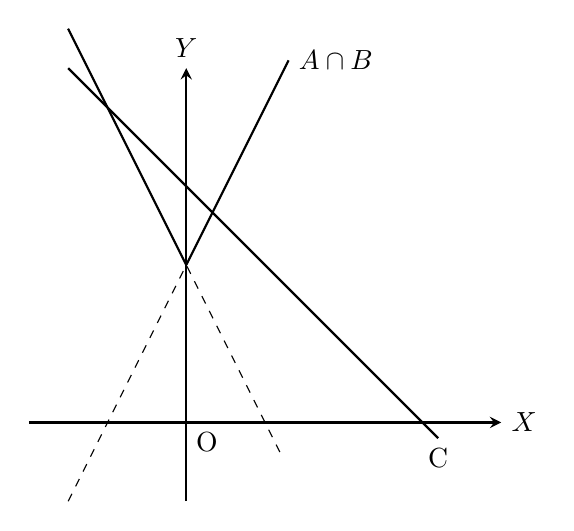
\begin{tikzpicture}[scale=1]
        \draw[thick,->,>=stealth](-2,0)--(4,0)node[right]{$X$};
        \draw[thick,->,>=stealth](0,-1)--(0,4.5)node[above]{$Y$};
        \node[below right]at(0,0){O};
        \draw[dashed,domain=-1.5:1.2]plot(\x,{-2*\x+2});
        \draw[thick,domain=-1.5:0]plot(\x,{-2*\x+2});
        \draw[dashed,domain=-1.5:1.3]plot(\x,{2*\x+2});
        \draw[thick,domain=0:1.3]plot(\x,{2*\x+2})node[right]{$A\cap B$};
        \draw[thick,domain=-1.5:3.2]plot(\x,{-\x+3})node[below]{C};
    \end{tikzpicture}
\end{center}
上図のCと$A\cap Bとの交点の座標を求めて,\\
\begin{cases}
    Y=-X+3\\
    Y=-2X+2
\end{cases}\doti(X,Y)=(-1,4)\\
\begin{cases}
    Y=-X+3\\
    Y=2X+2
\end{cases}\doti(X,Y)=(\dfrac{1}{3},\dfrac{8}{3})\\
\Y 求める交点の座標は,\kotaee{(x,y)=(-1,4),(\dfrac{1}{3},\dfrac{8}{3})}$
\newpage
\noindent{\LARGE \tokeni .}\\
\kai\\
まず,状況を整理するとこんな感じ.\\
\begin{center}
    \begin{tabular}{|c|c|c|c|}
        \hline
        $n$ & 1年目(100万) & 2年目(12万追加) & 3年目\\
        \hline 
        $S_n$ & $100\times1.08$ & $(108+12)\times1.08$ &{} \\
        \hline
        
    \end{tabular}
\end{center}
\tokeiichi  $\kotaee{S_1=108万円},\kotaee{S_2=129.6万}\\\\
\tokeini  \kotaee{S_{n+1}=\p{S_n+12}\times1.08 (n\geq1)}\cdots\asta \\\\
\tokeisan  特性方程式を解くことにより,\asta は次のように変形することができる.$
\begin{align*}
    \asta&\doti S_n+162=270\times\p{1.08}^{n-1}\\
    &\doti\kotaee{S_n=270\times\p{1.08}^{n-1}-162 (n\geq1)}
\end{align*}
\tokeishi \begin{align*} 
    \log10.8&=\log\dfrac{108}{10}=\log\dfrac{2^2\times3^3}{10}\\
    &=2\log2+3\log3-1=\kotaee{1.0333}
\end{align*}

\tokeigo  \begin{align*}
    S_n>513&\doti270\times\p{1.08}^{n-1}>512+513=675\\
    &\doti 1.08^{n-1}>\dfrac{5}{2}=\dfrac{10}{4}\\
    &\doti (n-1)\log1.08>\log\dfrac{10}{4}=1-2\log2=0.398\\
    &\doti0.0333(n-1)>0.398\\
    &\doti n-1>\dfrac{0.398}{0.0333}=11.9519\cdots\yaku11.95\\
    &\doti n>12.95
\end{align*}
$\Y 求める最小の自然数nは,\kotaee{13}$
\newpage
\noindent{\LARGE \tokesan.}\\
まず,与えられた状況を図示すると,下図のようになっている.
\begin{center}
    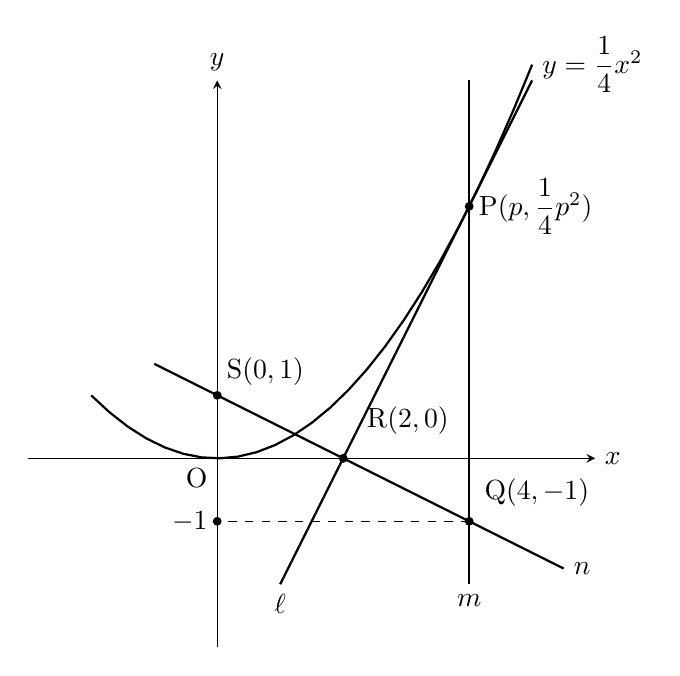
\begin{tikzpicture}[scale=0.8]
      \draw[->,>=stealth](-3,0)--(6,0)node[right]{$x$};
      \draw[->,>=stealth](0,-3)--(0,6)node[above]{$y$};
      \draw[thick,domain=-2:5] plot(\x,{pow(\x,2)/4})node[right]{$y=\dfrac{1}{4}x^2$};
      \coordinate[label=below left:O](O)at(0,0);

      \coordinate(P)at(4,4);
      \fill (P) circle (2pt);
      \node[right]at(P){P$(p,\dfrac{1}{4}p^2)$};

      \coordinate(R)at(2,0);
      \node[above right=2.5mm]at(R){R$(2,0)$};
      \fill (R) circle (2pt);

      \coordinate(S)at(0,1);
      \node[above right]at(S){S$(0,1)$};

      \fill(0,1)circle(2pt);

      \draw[thick,domain=2:5]plot(\x,{2*\x-4});
      \draw[thick,domain=2:1]plot(\x,{2*\x-4})node[below]{$\ell$};
      
      \draw[thick](4,6)--(4,-2)node[below]{$m$};
      \draw[thick,domain=-1:5.5]plot(\x,{-\x/2+1})node[right]{$n$};
      \draw[dashed](4,-1)--(0,-1);
      \node[left]at(0,-1){$-1$};
      \fill (0,-1)circle(2pt);
      \node[above right=1mm]at(4,-1){$\yad$Q$(4,-1)$};
      \fill(4,-1)circle(2pt);
     
    \end{tikzpicture}
\end{center}
\kai\\
$\mathrm{S}は,\mathrm{Q}の対称点であるから,座標は\mathrm{S}\p{0,1}とすぐに分かる.$\\
\tokeiichi  $y'=\dfrac{1}{2}xより,\ell の方程式は$
\begin{center}
    $\ell:y=\dfrac{1}{2}\p{x-p}+\dfrac{1}{4}p^2=\kotaee{\dfrac{1}{2}px-\dfrac{1}{4}p^2}$
\end{center}
\tokeini  $\mathrm{S}の座標は,\mathrm{S}(0,1)なので,nの方程式は,$
\begin{center}
    $n:y=\dfrac{-1-1}{p-0}(x-0)+1=\kotaee{-\dfrac{1}{p}x+1}$
\end{center}
Rの座標は,$\kotaee{\mathrm{R}(\dfrac{p}{2},0)}$\\\\
\tokeisan  Sの座標は点Qとの対称性より,\kotaee{0,1}\\\\
\tokeishi  $直線m'は,2点\mathrm{P},\mathrm{S}を通る直線であるから,$
\begin{center}
    $m':y=\dfrac{\dfrac{1}{4}p^2-1}{p-0}(x-0)+1$
\end{center}
$\Y \kotaee{m':y=\dfrac{p^2-4}{4}x+1}$\\
\newpage
\noindent 一方,Tは$Cとm'の共有点であるから,二次方程式:\dfrac{1}{4}x^2=\dfrac{p^2-4}{4p}x+1\doti(x-p)(px+4)=0を解くことにより,
x=p\vee x=-\dfrac{4}{p}を得るので,\mathrm{T}のx座標は,\kotaee{x=-\dfrac{4}{p}}$\\\\
\tokeigo  もとめる面積を$Lとおく.$
\begin{align*}
    L&=\dint{-\frac{4}{p}}{0}\p{\dfrac{p^2-4}{4p}x^2+x-\dfrac{1}{12}x^3}dx\\
    &=-\B{\dfrac{p^2-4}{8p}\tint{x^2}{-\frac{4}{p}}{0}+\tint{x}{-\frac{4}{p}}{0}-\dfrac{1}{12}\tint{x^3}{-\frac{4}{p}}{0}}\\
    &=\p{頑張って計算\cdots}\\
    &=\kotaee{\dfrac{6p^2+8}{3p^3}}
\end{align*}

\newpage
\subsection{2023年度2月9日実施}
{\LARGE \noindent\tokeichi.} \\
\kai\\
$\tokeiichi  余弦定理より,線分\mathrm{AD}について次のように2通りで表せる.\\
\mathrm{AD}^2=9+4-2\cdot3\cdot3\cdot2\cos A\cdots\maruichi\\
\mathrm{AD}^2=25+36-2\cdot5\cdot6\cos A\p{\pi-A}=25+36+2\cdot5\cdot6\cos A\cdots\maruichi\\
\Y \maruichi と\maruni より,25+36+60\cos A=9+4-12\cos A\doti72\cos A=-48\\
\Y \kotaee{\cos A=-\dfrac{2}{3}}\\\\
\tokeini  (x+1)^{2023}について,二項定理より,\\
(x+1)^{2023}=\comb{2023}{1}+\comb{2023}{1}x+\wa{k=2}{2023}\comb{2023}{k}x^k\godo\kotaee{1+2023x}\pmod{x^2}\\\\$
\tokeisan  \begin{align*}
    \dfrac{1}{1-a}&=\dfrac{1}{1-\log_62}=\dfrac{1}{\log_66-\log_62}\\
    &=\dfrac{1}{\log63}=\dfrac{1}{\dfrac{\log_33}{\log_36}}=\log_36
\end{align*}
$\Y 3^{\dfrac{1}{1-a}}=3^{\log_36}=\kotaee{6}$\\\\
\tokeishi  $3点\mathrm{O},\mathrm{A},\mathrm{B}を通る円の方程式は,x^2+y^2+ax+by+c=0\cdots\asta とかける.\\
これより,$
\begin{align*}
    \begin{cases}
        c=0\\
        -6a+6b=-72\\
        4a+2b=-20
    \end{cases}&\doti\begin{cases}
        c=0\\
        a-b=12\\
        2a+b=-10
    \end{cases}\\
    &\doti\begin{cases}
        a=2/3\\
        b=-34-3\\
        c=0
    \end{cases}
\end{align*}
$\Y x^2+y^2+\dfrac{2}{3}x-\dfrac{34}{3}y=0\\\
\Y \p{x+\dfrac{1}{3}}^2+\p{y-\dfrac{17}{3}}^2=\cdots\\
\Y 円の中心の座標は,\kotaee{\p{-\dfrac{1}{3},\dfrac{17}{3}}}$
\newpage
\noindent\tokeigo  $z=\dfrac{\sqrt{3}}{2}+\dfrac{i}{2}において,z=r\p{\cos\theta+i\sin\theta}(r>0)とおくと,\\
z=\cos\dfrac{\pi}{6}+i\sin\dfrac{\pi}{6}なので,\\
z^6=\cos\pi+i\sin\pi=-1\\
\Y\kotaee{\begin{cases}
    a=-1\\
    b=0
\end{cases}}$\\\\
\tokeiroku  \begin{align*}
&\left|\vec{a}+\vec{b}\right|=\sqrt{17}\doti2\vec{a}\cdot\vec{b}=-8\\
&\doti\vec{a}\cdot\vec{b}=-4
\end{align*}
$\Y S=\sqrt{9\cdot16-(-4)^2}=\kotaee{8\sqrt{2}}\\\\$
\tokeishichi  $a_1=0,a_2=3,a_3=0,\cdots\\
と続くような漸化式なので,n=2m  または, n=2m+1と表すことができる.\\
\Y \wa{k=1}{2m}a_k=\overbrace{0+3+0+3+\cdots}^{2m個}=(3がm個)=3m\\
一方,\wa{k=1}{2m+1}a_k=\overbrace{0+3+0+3+\cdots}^{2m個}+0=(3がm個+0)=3m\\
\Y いずれのときも,\wa{k=1}{n}a_k=\kotaee{3m}$
\newpage
\noindent{\LARGE \tokeni.}\\
\kai\\
\tokeiichi  (A,B,C,D)の手の出し方は,次の3通りである.\\
(A,B,C,D)$=$(グ,チ,チ,チ),(チ,パ,パ,パ),(パ,グ,グ,グ)\\
$\Y 求める確率は,\dfrac{3}{3^4}=\kotaee{\dfrac{1}{27}}$\\\\
\tokeini  A以外の勝者の決め方は,$\comb{3}{1}=3通りであり,二人のみ勝つ場合は,3通りである.\\
\Y 求める確率は,\dfrac{3\times3}{3^4}=\kotaee{\dfrac{1}{9}}$\\\\
\tokeisan  \tokeiichi で,Aが一人で勝つ場合,\tokeini でAとその他一人が勝つ場合を求めているので,あとはAと他二人が勝つ場合を求めれば良い.
他二人の選び方は,$\comb{3}{2}=3通りであり,手の出し方が3通りある.\\
\Y 求める確率は,\tokeiichi と\tokeini の結果を合わせて,\dfrac{3+9+9}{3^4}=\kotaee{\dfrac{7}{27}}$\\\\
\tokeishi  あいこが発生するのは,「全員が同じ手」と「4人の内3人が違う手」である.\\
まず,前者の場合から考える.\\
・\underline{全員が同じ手になる確率}\\
 これは,明らかに$\dfrac{3}{3^4}\cdots\cdots\maruichi $である.\\
・\underline{4人の内3人が違う手になる確率}\\
 3人の内,2人の手が決まれば,残り1人の手の出し方は,ただ一通りなので,先にその二人を指定する.\\
$二人の選び方\to\comb{4}{2}=6通り.また,3人の内のもう一人の手の出し方は1通り.最後に,4人目の人の手の出し方は,3通り.\\
ここで,三人目の人と4人目の人の並び方を考えて,2!=2通りである.\\
\Y このときの確率は,\dfrac{\comb{4}{2}\times1\times3\times2}{3^4}=\dfrac{36}{3^4}\cdots\cdots\maruni である.\\
\Y 以上より,求める確率は,\maruichi+\maruni=\dfrac{39}{3^4}=\kotaee{\dfrac{13}{27}}$\\\\
\tokeigo  2回目でゲームが終了するのは,\ans{1回目があいこで,2回目で少なくとも一人勝つとき}である.\\
従って,あいこになる確率は\tokeishi で求めているので,4人の内少なくとも1人勝つ確率を求めて,これらの積を考えれば良い.\\
ここで,「4人の内少なくとも一人勝つ」$\doti 「1-\p{あいこになる確率}」である.即ち,あいこの余事象である.\\
\Y 求める確率は,\dfrac{13}{27}\times\dfrac{14}{27}=\kotaee{\dfrac{13\times14}{27^2}}$
\newpage
\noindent{\LARGE\tokesan.}\\
\begin{center}
    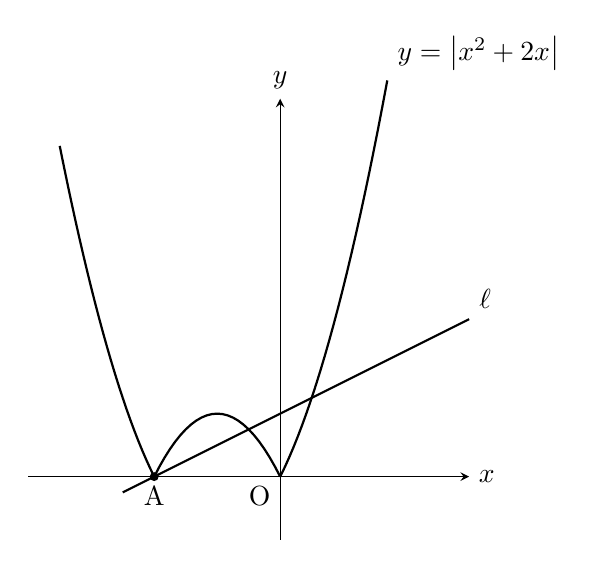
\begin{tikzpicture}[scale=0.8]
        \draw[->,>=stealth](-4,0)--(3,0)node[right]{$x$};
        \draw[->,>=stealth](0,-1)--(0,6)node[above]{$y$};
        \draw[thick,domain=-3.5:-2] plot(\x,{pow(\x,2)+2*\x});
        \draw[thick,domain=-2:0] plot(\x,{-pow(\x,2)-2*\x});
        \draw[thick,domain=0:1.7] plot(\x,{pow(\x,2)+2*\x})node[above right]{$y=\left|x^2+2x\right|$};

        \coordinate[label=below left:O](O)at(0,0);

        \coordinate[label=below:A](A)at(-2,0);
        \fill (A)circle(2pt);

        

        
        \draw[thick,domain=-2.5:3] plot(\x,{\x/2+1})node[above right]{$\ell$};




    \end{tikzpicture}
\end{center}
\kai\\
\tokeiichi  $\mathrm{A}(-2,0)を通る傾きtの直線の方程式は,\ell:y=tx+2t\cdots\cdots\maruichi  とかける.$\\
 また,2点P,Qの座標は,
 \begin{align*}
    \left|x^2+2x\right|=tx+2t&\doti x^2+2x=tx+2t\vee x^2+2x=-(tx+2t)\\
    &\doti x^2+(2-t)x-2t=0\vee x^2+(2+t)x+2t=0\\
    &\doti (x-t)(x+2)=0\vee (x+t)(x+2)=0\\
    &\doti \p{x=t\vee x=-2}\vee\p{x=-t\vee x=0}
 \end{align*}
$\Y \mathrm{P}のx座標は\mathrm{Q}のy座標より小さいので,\kotaee{\mathrm{P}_x=-t,\mathrm{Q}_x=t}$\\\\
\tokeini  \begin{align*}
S_1(t)&=\dint{-2}{-t}\B{-(x^2+2x)-t(x+2)}dx\\
&=-\dint{-2}{-t}(x+2)(x+t)dx\\
&=\dfrac{1}{6}\p{-t+2}^3
\end{align*}
$\Y \kotaee{S_1(t)=\dfrac{1}{6}(2-t)^3}$\\\\
\tokeisan  \begin{align*}
    S_2(t)&=\dint{-t}{0}\B{t(x+2)-(-x^2-2x)}dx+\dint{0}{t}\B{t(x+2)-(x^2-2x)}dx\\
    &=\dint{-t}{0}\B{x^2+(2+t)x+2t}dx+\dint{0}{t}\B{-x^2+(t-2)x+2t}dx\\
    &=\dfrac{1}{3}\tint{x^3}{-t}{0}-\dfrac{1}{3}\tint{x^3}{0}{t}+\dfrac{2+t}{2}\tint{x^2}{-t}{0}+\dfrac{t-2}{2}\tint{x^2}{t}{0}
    +2t(0+t)+2t(t-0)\\
    &=\dfrac{t^3}{3}-\dfrac{t^3}{3}-\dfrac{t+2}{2}t^2+\dfrac{t-2}{2}t^2+2t^2+2t^2\\
    &=\kotaee{2t^2}
\end{align*}\\
\tokeishi  \tokeini と\tokeisan の結果より,$\kotaee{S(t)=\dfrac{1}{6}(2-t)^3+2t^2\cdots\cdots\maruni}$\\
ここで,$\maruni に積の微分法を用いて微分すると,$
\begin{align*}
    \dfrac{d}{dt}S(t)&=\dfrac{1}{2}(2-t)^2\times(-1)+4t\\
    &=\kotaee{-\dfrac{1}{2}(2-t)^2+4t}
\end{align*}
\newpage
\noindent\tokeigo  $\tokeishi より,\dfrac{d}{dt}S(t)=0を解くと,0<t<2に注意して,t=6-4\sqrt{2}を得る.これを\alpha とおく.\\
このとき,以下の増減表を得る.$
\begin{center}
    \begin{tabular}{|c||c|c|c|c|c|}
        \hline
        $t$ & 0 & $\cdots$ & $\alpha$ & $\cdots$ & 2\\
        \hline
        $\dfrac{dS(t)}{dt}$ &  & $-$ & 0 & $+$ & \\
        \hline
        $S(t)$ & & $\yab$ & $S(\alpha)$ & $\yaa$ & \\
        \hline
    \end{tabular}
\end{center}
$\Y S(t)を最小にするようなtの値は,\kotaee{t=6-4\sqrt{2}}$

\newpage
\subsection{2024年度2月6日実施}
\noindent{\LARGE\tokeichi.}\\
\kai\\
\tokeiichi  $t=\log_2x とおくと,y=t^2-8t-20\cdots\cdots\maruichi なので,y'=2t-8より,\\
\maruichi はt=4\doti x=16 のとき,最小値をとるので,1\leq x\leq8 より,\kotaee{x=8}(:\Bc{ア})のとき,\min y=\kotaee{-35}(:\Bc{イ}).\\\\
\tokeini  両辺に(x+1)^3をかけることにより,$
   \begin{align*}
    3x^2-x+4&=a+b(x+1)+c(x+1)^2\\
    &=cx^2+(b+2c)x+a+b+c\cdots\cdots\maruichi 
   \end{align*} 
ここで,$\maruichi$ は等式として一致するので,両辺の係数を比較することにより,\\
$\begin{cases}
c=3\\
b+2c=-1\\
a+b+c=4
\end{cases}\doti\kotaee{\begin{cases}
    a=8\\
    b=-7\\
    c=3
\end{cases}}$\\\\
\tokeisan  「さいころを3回投げて,出る目の積が4の倍数」$\doti$ 「少なくとも1回4の倍数が出る.」\\
このことより,\ans{3回とも1,3,5のどれか.}と\ans{4以外の偶数の目が1回だけでる.}場合の確率を求めて,余事象を考えれば良い.\\
・\underline{3回とも1,3,5のどれかがでるとき,}\\
 この場合の確率は,$\p{\dfrac{3}{6}}^3\cdots\cdots\maruichi  である.$\\
・\underline{4以外の偶数の目が1回だけでるとき,}\\
  $この場合の確率は,\comb{3}{1}\p{\dfrac{2}{6}}\p{\dfrac{3}{6}}^2=\dfrac{54}{6^3}\cdots\cdots\maruni  である.$\\
$\Y \maruichi,\maruni より求める確率は,1-\dfrac{81}{6^3}=1-\dfrac{3}{8}=\kotaee{\dfrac{5}{8}}$
\newpage
\noindent\tokeishi  $ここで,一般の角\alpha,\beta について\tan の加法定理を考えると,次式で表される.$
\begin{center}
    $\tan\p{\alpha\pm\beta}=\dfrac{\tan\alpha\pm\tan\beta}{1\mp\tan\alpha\tan\beta}
    =\dfrac{1\pm\dfrac{\tan\beta}{\tan\alpha}}{\dfrac{1}{\tan\alpha}\mp\tan\beta}\cdots\cdots\asta $
\end{center}
これに注目すると,与えられた式は,\ans{\asta の分母}であるから,$\asta で\beta=\alpha とおくと,$
\begin{align*}
    \tan\p{2\alpha}&=\dfrac{1+1}{\dfrac{1}{\tan\alpha}-\tan\alpha}\\
    &=\dfrac{2}{\dfrac{1}{\tan\alpha}-\tan\alpha}\\
    &\doti \dfrac{1}{\tan\alpha}-\tan\alpha=\left.\dfrac{2}{\tan2\alpha}\right|_{\alpha=\dfrac{\pi}{12}}
    =\kotaee{2\sqrt{3}}
\end{align*}\\
\tokeigo  少し数列の構造を調べてみよう.
\begin{center}
    \begin{tabular}{|c||c|c|c|c|c|c|}
        \hline
        $n$ & $1$ & $2$ & $3$ & $4$ & $5$ & $\cdots$\\
        \hline
        $a_n$ & 1 & 1 & 2 & 4 & 8 & $\cdots$\\
        \hline
        
    \end{tabular}
\end{center}
このことから,数列の構造は以下のようになっている.
\begin{center}
    

$1,1\to^{\times2}2\to^{\times2}4\to^{\times2},\cdots,\to^{\times2(n-2回目)}a_n$
\end{center}
$\Y 一般項a_nは,\kotaee{a_n=2^{n-2}}である.(これは,n\geq3のとき確かに成立している.)$\\\\
\tokeiroku  $f(x)\p{\dint{0}{1}f(t)dt}=x^2+5\cdots\cdots\asta\\
    今, A=\dint{0}{1}f(t)dtとおくと,Aは定数なので,f(t)=\dfrac{t^2+5}{A}であるから,$
    \begin{align*}
        A&=\dint{0}{1}\dfrac{1}{A}\p{t^2+5}dt=\dfrac{1}{A}(\dfrac{1}{3}+5)(積分計算は省略)\\
        &=\dfrac{16}{3}\cdot\dfrac{1}{A}\\
        &\doti A=\pm\dfrac{4}{\sqrt{3}}
    \end{align*}
    $\Y A>0より,A=\dfrac{4}{\sqrt{3}}\\
    \Y f(x)=\dfrac{\sqrt{3}}{4}x^2+\dfrac{\sqrt{3}}{4}\cdot5\\
    \Y \kotaee{a=\dfrac{\sqrt{3}}{4},b=\dfrac{5\sqrt{3}}{4}}$
\newpage
\noindent{\LARGE\tokeni.}\\
\kai\\
まず,与えられた状況を図示すると以下のようになる.\\
{tikzpicture スペース}\\
\tokeiichi  $ y'=-2xより,\\
\ell:y=-2p(x-p)-p^2=\kotaee{-2px+p^2}\\
m:y=2q(x+q)-q^2=\kotaee{2qx+q^2}$\\\\
\tokeini   $\ell とmの交点を求めれば良いので,\\
\begin{cases}
    y=-2px+p^2\\
    y=2qx+q^2
\end{cases}\doti\begin{cases}
    x=\dfrac{p^2-q^2}{2(p+q)}=\dfrac{p+q}{2}\\
    y=pq
\end{cases}\\
\Y \kotaee{\mathrm{R}\p{\dfrac{p-q}{2},pq}}$\\\\
\tokeisan  $\mathrm{Q}\p{-q,-q^2},\ell:y=-2px+p^2より、点と直線の距離公式から,$
\begin{align*}
    d&=\dfrac{\left|-2pq-q^2-p^2\right|}{\sqrt{(2p)^2+1^2}}\\
    &=\dfrac{\left|2pq+q^2+p^2\right|}{\sqrt{4p^2+1}}\\
    &=\kotaee{\dfrac{(p+q)^2}{\sqrt{4p^2+1}}}
\end{align*}
\tokeishi  まず,高さに相当するPRを求める.$\Vec{PR}=\tvec<0,1>[-\dfrac{1}{2}(p+q),p(q+p)]より,$
\begin{align*}
    \left|\Vec{PR}\right|&=\sqrt{\dfrac{1}{4}(p+q)^2+p^2(q+p)^2}\\
    &=(p+q)\sqrt{\dfrac{1}{4}+p^2}\\
    &=\dfrac{p+q}{2}\sqrt{4p^2+1}
\end{align*}
このことより,求める面積Sは
\begin{align*}
    S&=\dfrac{1}{2}\times\left|\Vec{PR}\right|\times d\\
    &=\dfrac{1}{2}\cdot\dfrac{p+q}{2}\sqrt{4p^2+1}\cdot\dfrac{(p+q)^2}{\sqrt{4p^2+1}}\\
    &=\kotaee{\dfrac{1}{4}(p+q)^3}
\end{align*}
\newpage
\noindent\tokeigo  $2直線\ell,mが直交するので,(-2p)(2q)=-1\doti\kotaee{q=\dfrac{1}{4p}}$\\\\
\tokeiroku  $\tokeigo を用いると,面積\mathrm{S}は,S=\dfrac{1}{4}(p+\dfrac{1}{4p})\cdots\cdots\asta とかけるので,
\asta に\mathrm{AM-GM}の関係を用いると,$
\begin{center}
    $p+\dfrac{1}{4p}\geq2\sqrt{p\cdot\dfrac{1}{4p}}=1$
\end{center}
等号成立は,$p=\dfrac{1}{4p}\doti p=\dfrac{1}{2}のとき成立する.(\because p>0)$\\ 
$\Y 求める最小値は,\min S=\kotaee{\dfrac{1}{4}},またそのときのpはp=\kotaee{\dfrac{1}{2}}である.$
\newpage
\noindent{\LARGE\tokesan.}\\
tikzpicture でお絵描きできなかった(技量不足)ので,板書よくみといてください!\hiraayamari\\
\kai\\
$\tokeiichi  余弦定理より,\cos\Kaku{AOB}=\dfrac{25+49-64}{2\cdot5\cdot7}=\dfrac{1}{7}.\\
\Y \vec{a}\cdot\vec{b}=35\cdot\dfrac{1}{7}=\kotaee{5}\\\\$
\tokeini  余弦定理より,$\cos\Kaku{OAB}=\dfrac{8^2+5^2-7^2}{2\cdot5\cdot8}=\dfrac{40}{80}=\dfrac{1}{2}なので,\\
\mathrm{AD}=\mathrm{OA}\cos60^{\ddo}=5\cdot\dfrac{1}{2}=\dfrac{5}{2}\\$
このとき,$\mathrm{BD}=8-\dfrac{5}{2}=\dfrac{11}{2}なので,\mathrm{AD}:\mathrm{BD}=5:11であるから,$
\begin{center}
    $\Vec{OD}=\dfrac{11\Vec{OA}+5\Vec{OB}}{5+11}=\dfrac{11}{16}\Vec{OA}+\dfrac{5}{16}\Vec{OB}$
    \end{center}
    $\Y \kotaee{t=\dfrac{5}{16}}$\\\\
    \tokeisan  $\mathrm{OD}=\mathrm{OA}\cos60^{\ddo}=\dfrac{5\sqrt{3}}{2}\\
    \Y 半径r=\kotaee{\dfrac{5\sqrt{3}}{2}}$\\\\
    \tokeishi  \begin{align*}
    \Vec{OH}&=\p{\Vec{OD}の\vec{a}向き正射影ベクトル}=\dfrac{\Vec{OD}\cdot\vec{a}}{\left|\vec{a}\right|^2}\vec{a}\\
    &=\dfrac{\dfrac{11}{16}\left|\vec{a}\right|^2+\dfrac{5}{16}\vec{a}\cdot\vec{b}}{25}\vec{a}
    =\dfrac{\dfrac{11\cdot25}{16}+\dfrac{25}{16}}{25}\vec{a}\\
    &=\dfrac{11+1}{16}\vec{a}=\kotaee{\dfrac{3}{4}\vec{a}}
    \end{align*}\\
\tokeigo  \fbox{コメント}:$\Vec{OH}が使えたら嬉しい.$\\
円の幾何学的性質より,$点\mathrm{H}は線分\mathrm{DE}の中点であるから,\Vec{OH}=\dfrac{\Vec{OD}+\Vec{OE}}{2}\cdots\cdots\maruichi  を満たす.\\
このことより,$
\begin{align*}
    \Vec{OE}&=2\Vec{OH}-\Vec{OD}=\dfrac{3}{2}\vec{a}-\p{\dfrac{11}{16}\vec{a}+\dfrac{5}{16}\vec{b}}\\
    &=\dfrac{13}{16}\vec{a}-\dfrac{5}{16}\vec{b}
\end{align*}
$\Y \kotaee{p=\dfrac{13}{16},q=-\dfrac{5}{16}}$
\newpage
\begin{center}
    {\LARGE 傾向と対策の補足}
\end{center}

\begin{center}
        \begin{tabular}{|c|c|c|}
            \hline
           {}&  \tokeni & \tokesan \\
           \hline
           2018 & \suII 三角関数と微積 & \suB ベクトル\\
           \hline
           2019 & \suII 微積 & \suII 図形と方程式\\
           \hline
           2020 & \suII 微積 & \suA\suII 三角関数と整数\\
            \hline
            2023.2/6 & \suB 複利計算 & \suII 微積\\
            \hline
            2023.2/9 & \suA 確率 & \suI\suII 絶対値のついた二次関数,微積\\
            \hline
            2024.2/6 & \suII 微積 & \suC ベクトル\\
            \hline 
            2024.2/9 & \suB 漸化式 & \suI\suII 二次関数と微積\\
            \hline
            2025.2/6 & \suA\suB 確率漸化式 & \suII 微積\\
            \hline
            2025.2/9 & \suII 三角関数と図形の融合問題 & \suII 微積\\
            \hline
        \end{tabular}
    \end{center}







\end{document} 